\section{Tutorial -- Creating a Flowsheet}\label{tutorial.simple.flow}

This tutorial provides information about the basic use of FOQUS and setting up a very simple flowsheet.  A single node flowsheet will be created that performs a simple calculation using a square root so that simulation errors can be observed when a negative input value is provided.

\begin{enumerate}
	\item Start FOQUS (see Section \ref{sec.flowsheet.starting.foqus}).
	\item In the session form enter the \textbf{\underline{Session Name}} as ``Simple\_Flow'' (Figure \ref{fig.session.name1}).
\end{enumerate}

\begin{figure}[H]
	\begin{center}
		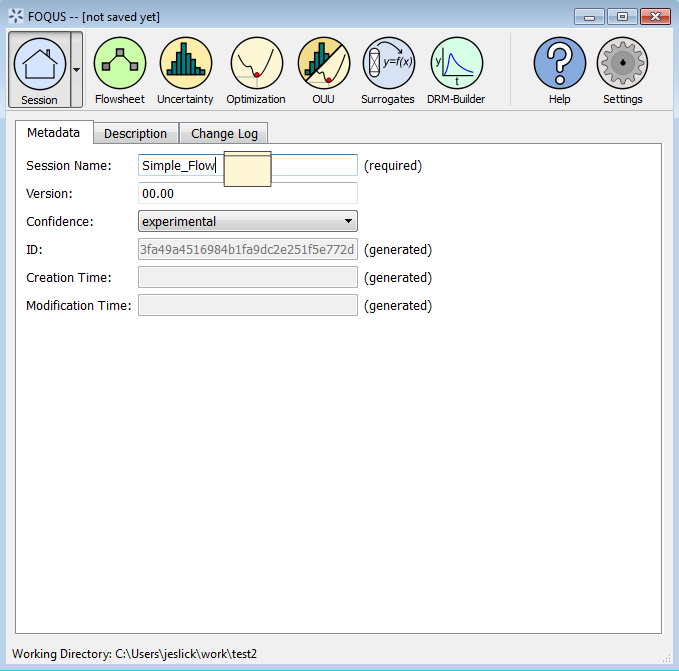
\includegraphics[scale=0.55]{Chapt_flowsheet/figs/session_name1}
		\caption{Setting the Session Name}
		\label{fig.session.name1}
	\end{center}
\end{figure}

\begin{enumerate}
	\setcounter{enumi}{2}
	\item Set the session description.
	\begin{enumerate}
		\item Select the \bu{Description} tab (Figure \ref{fig.session.description1}).
		\item Type the description shown in Figure \ref{fig.session.description1}.  The buttons above the \textbf{\underline{Description}} tab box can be used to format the text.
	\end{enumerate}
\end{enumerate}

\begin{figure}[H]
	\begin{center}
		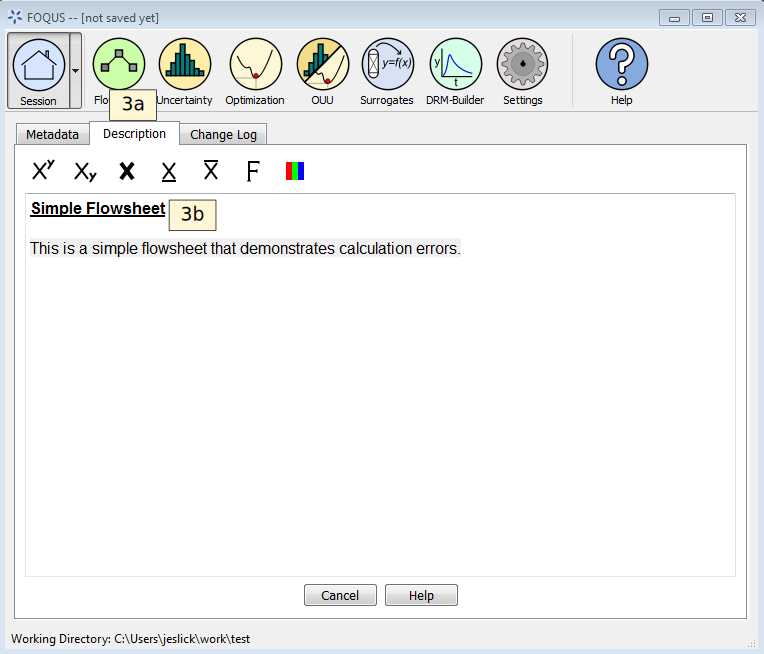
\includegraphics[scale=0.55]{Chapt_flowsheet/figs/session_description1}
		\caption{Setting the Session Description}
		\label{fig.session.description1}
	\end{center}
\end{figure}


\begin{enumerate}
	\setcounter{enumi}{3}
	\item Click the \textbf{\underline{Flowsheet}} button at the top of the Home window (Figure \ref{fig.simple.flow1}).
	\item Add a node named ``calc.''
	\begin{enumerate}
		\item Click the \textbf{\underline{Add Node}} button in the toolbar on the left side of the Home window.
		\item Click a location on the gridded flowsheet area.
		\item Enter the node name ``calc'' in the dialog box.
	\end{enumerate}
	\item Click the \textbf{\underline{Select Mode}} button in the toolbar.
	\item Open the Node Editor by clicking the \textbf{\underline{Node Editor}} button in the toolbar.
	\item Add input variables to the node. (When linking a node to an external simulation the input and output variables are populated automatically, and this step is not necessary.)
	\begin{enumerate}
		\item Click \bu{+} above the \textbf{\underline{Input Variables}} table.
		\item Enter x1 in the variable \textbf{\underline{Name}} dialog box.
		\item Click \bu{+} above the \textbf{\underline{Input Variables}} table.
		\item Enter x2 in the variable \textbf{\underline{Name}} dialog box.
		\item Enter -2 and 2 for the \textbf{\underline{Min}} and \textbf{\underline{Max}} of x1 in the \textbf{\underline{Input Variables}} table.
		\item Enter -1 and 4 for the \textbf{\underline{Min}} and \textbf{\underline{Max}} of x2 in the \textbf{\underline{Input Variables}} table.
		\item Enter 1 for the value of x1.
		\item Enter 4 for the value of x2.
	\end{enumerate}
\end{enumerate}

\begin{figure}[H]
	\begin{center}
		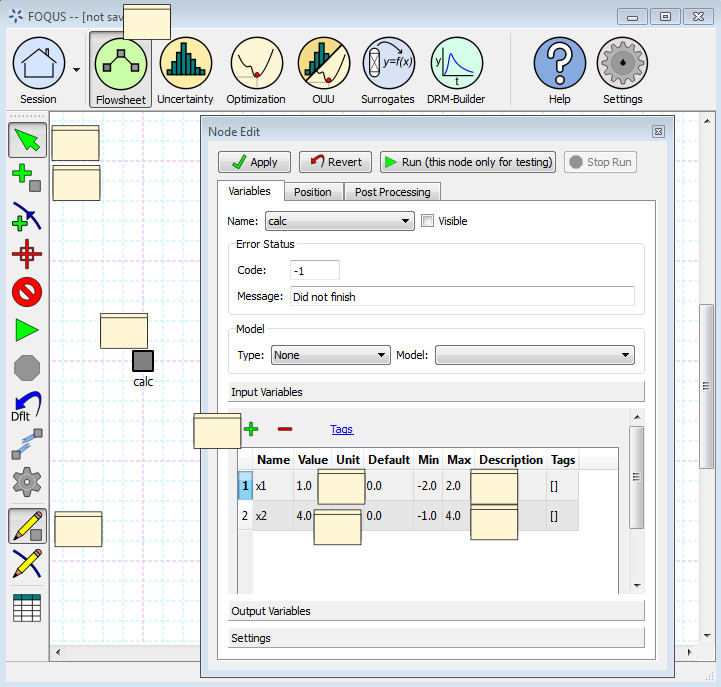
\includegraphics[scale=0.55]{Chapt_flowsheet/figs/simple_flow_1}
		\caption{Flowsheet, Input Variables}
		\label{fig.simple.flow1}
	\end{center}
\end{figure}

\begin{enumerate}
	\setcounter{enumi}{8}
	\item Add an output variable to the node. (When linking a node to an external simulation the input and output variables are populated automatically.)
	\begin{enumerate}
		\item Click \bu{Output Variables} to show the \textbf{\underline{Output Variables}} table (Figure \ref{fig.simple.flow2}).
		\item Click \bu{+} above the \textbf{\underline{Output Variables}} table to add a variable.
		\item Enter z in the output \textbf{\underline{Name}} dialog box.
	\end{enumerate}
\end{enumerate}

\begin{figure}[H]
	\begin{center}
		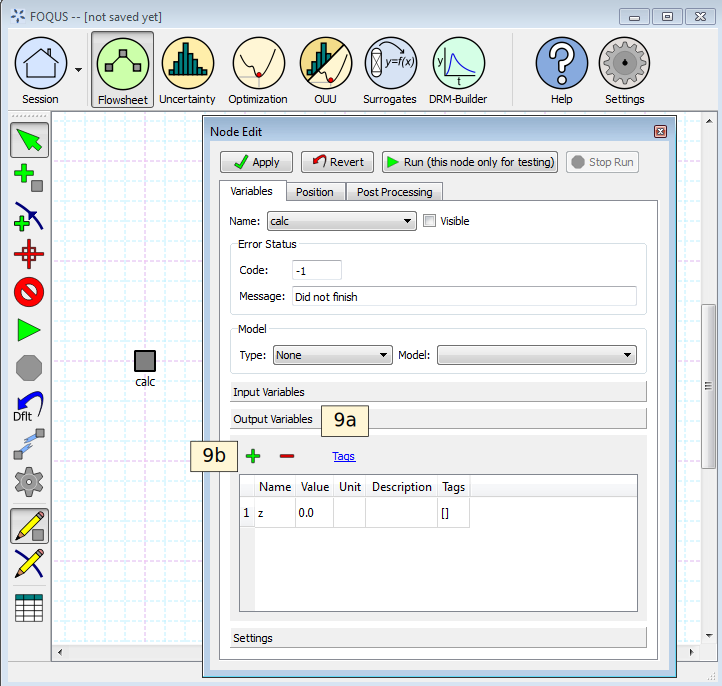
\includegraphics[scale=0.55]{Chapt_flowsheet/figs/simple_flow_2}
		\caption{Flowsheet, Output Variables}
		\label{fig.simple.flow2}
	\end{center}
\end{figure}

In this example, the node is not linked to any external simulation. The FOQUS nodes contain a section called node script, which can be used to do calculations before, after or instead of a simulation linked to the node. The node script can be used for things such as unit conversion, simple calculations, or simulation convergence procedures. The node scripts are written as Python. The \textbf{\underline{Input Variables}} are contained in a dictionary named x and the \textbf{\underline{Output Variables}} are contained in a dictionary named f. The dictionary keys are the variables names shown in the input and output tables. Only \textbf{\underline{Output Variables}} can be modified by a node script.

\begin{enumerate}
	\setcounter{enumi}{9}
	\item Add a calculation to the node.
	\begin{enumerate}
		\item Click the \bu{Node Script} tab (Figure \ref{fig.simple.flow3}).
		\item Enter the following code into the Python code box: \\ \verb|f['z'] = x['x1']*math.sqrt(x['x2'])|
	\end{enumerate}
	\item Click the \bu{Variables} tab.
	\item Click the \textbf{\underline{Run}} button (Figure \ref{fig.simple.flow3}).
\end{enumerate}

The flowsheet should run successfully and the output value should be 2. Rerun the flowsheet with a negative value for x2, and observe the result. The simulation should report an error.

\begin{figure}[H]
	\begin{center}
		\includegraphics[scale=0.55]{Chapt_flowsheet/figs/simple_flow_3}
		\caption{Node Calculation}
		\label{fig.simple.flow3}
	\end{center}
\end{figure}

\begin{enumerate}
	\setcounter{enumi}{9}
	\item Save the FOQUS session.
	\begin{enumerate}
		\item Click the \bu{Session} drop-down menu at the top of the Home window (Figure \ref{fig.simple.flow.save}).
		\item Click \bu{Save}. The exact location of save in the menu depends on whether or not the data management framework is enabled.
		\item The \textbf{\underline{Change Log}} entry can be left blank.
		\item The default file name is the session name. Change the file name and location if desired.
	\end{enumerate}
\end{enumerate}

\begin{figure}[H]
	\begin{center}
		\includegraphics[scale=0.55]{Chapt_flowsheet/figs/simple_flow_save}
		\caption{Save Session}
		\label{fig.simple.flow.save}
	\end{center}
\end{figure}


